\documentclass[CJKmath]{ctexart}
\usepackage{geometry}
\geometry{inner=1.45cm,outer=2.45cm,top=2.45cm,bottom=3cm}
\RequirePackage[dvipsnames,svgnames,x11names,table]{xcolor}

\usepackage{xeboiboites}
% /* --------------------------------- 模板默认颜色 --------------------------------- */
\colorlet{outermarginfgcolor}{DarkCyan} % foregroundcolor 较深的前景色
\colorlet{outermarginbgcolor}{DarkCyan!30} % backgroundcolor 较浅的背景色
% /* -------------------------------------------------------------------------- */

\RequirePackage{tikz,calc} %%页面样式设计核心包 %提供\pgfonlayer命令
\usetikzlibrary{cd,calc,shadows,hobby,intersections, decorations.markings, decorations.pathreplacing,spy,arrows,shapes,fadings,trees,mindmap,patterns,shapes.arrows,shapes.symbols,tikzmark,shapes.geometric,graphs, quotes, angles,decorations.pathmorphing,through,shadings,backgrounds,positioning,fit,arrows.meta,shapes.misc,decorations.shapes}

% 绘图:函数图像
\usepackage{pgfplots}
\pgfplotsset{compat=1.18}

\RequirePackage[most]{tcolorbox}
\tcbuselibrary{breakable, skins,theorems}


\usepackage{amsmath,amssymb}
\usepackage{xparse}
\usepackage{etoolbox}
\RequirePackage[explicit]{titlesec}
\usepackage{varwidth}
% /* -------------------------------- Section样式 ------------------------------- */
\titleformat{\section}
{\thispagestyle{empty}}
{}
{-.5em} %左右移动\thesection标签位置
{\mysectionformat{#1}}

\titleformat{name=\section,numberless}{}{}{-.5em}{\mysectionnonumformat{#1}}

\newcommand{\mysectionformat}[1]{%
\makebox[0pt][l]{\def\rad{7pt}%
\begin{tikzpicture}[remember picture]
%  \path[fill=outermarginfgcolor,drop shadow={opacity=0.3,shadow xshift=.05cm,shadow yshift=-.05cm}]node[append after command={
%  (sec.north west) -- (sec.south west) -- ([xshift=-\rad]sec.south east) to[out=0,in=180,looseness=1] ([xshift=3*\rad]sec.north east) --cycle},
%  text=white,font=\sffamily\large\bfseries,align=center,inner ysep=2mm] (sec) at (0,0) {\thesection};
	\path[fill=outermarginfgcolor,drop shadow={opacity=0.2,shadow xshift=.05cm,shadow yshift=-.05cm}]node[append after command={
  (sec.north west) -- (sec.south west) -- ([xshift=-\rad]sec.south east) to[out=0,in=180,looseness=0] ([xshift=1*\rad]sec.north east) --cycle},
  text=white,font=\sffamily\large\bfseries,align=center,inner ysep=2mm] (sec) at (0,0) {\thesection};
  % 标题
  \path[fill=outermarginfgcolor,drop shadow={opacity=0.2,shadow xshift=.05cm,shadow yshift=-.05cm}]node[append after command={
      ([xshift=1*\rad]secnum.north west) to[out=180,in=0,looseness=0] ([xshift=-1*\rad]secnum.south west) --(secnum.south east) to (secnum.north east) --cycle},text=black,font=\sffamily\large\bfseries,below right](secnum) at ([shift={(.5*\rad,-0.5mm)}]sec.north east) {\begin{varwidth}{.85\linewidth}\setlength\baselineskip{18pt}\hspace{.5cm}#1\end{varwidth}};
\end{tikzpicture}}}%最后一个选项为 [<after code>]

\newcommand{\mysectionnonumformat}[1]{%
\makebox[0pt][l]{\def\rad{7pt}%
\begin{tikzpicture}[remember picture]
  \path[fill=outermarginfgcolor,drop shadow={opacity=0.3,shadow xshift=.05cm,shadow yshift=-.05cm}]node[append after command={
  % 去掉左侧曲线,改为直线;右侧保持原先弧线造型
  (sec.north west) -- (sec.south west) -- ([xshift=-\rad]sec.south east) to[out=0,in=180,looseness=1] ([xshift=3*\rad]sec.north east) --cycle},
  text=white,font=\sffamily\large\bfseries,align=center,inner ysep=2mm] (sec) at (0,0) {Sec};
  \node[text=black,font=\large,below right] (secnum) at ([shift={(0,-1mm)}]sec.north east) {\begin{varwidth}{.85\linewidth}\setlength\baselineskip{18pt}\hspace{.5cm}#1\end{varwidth}};
\end{tikzpicture}}}%最后一个选项为 [<after code>]

\titlespacing*{\section}{0pt}{3.5ex plus 1ex minus .2ex}{2.3ex plus .2ex}


% ==== ElegantBook fancy-mode exercise (standalone) ====
\makeatletter
\newcommand{\exercisename}{}
\definecolor{main}{RGB}{0,120,2}
\colorlet{outermarginfgcolor}{DarkCyan} % foregroundcolor 较深的前景色
\colorlet{outermarginbgcolor}{white} % backgroundcolor 较浅的背景色
% 设定主编号上级计数器(tcolorbox auto counter 使用)
\def\ELEGANT@thmcnt{section}

\tcbset{new/usesamecnt/.style={}}

\tcbset{
  common/.style={
    fontupper=\itshape,
    lower separated=false,
    coltitle=white,
    colback=gray!5,
    boxrule=0.5pt,
    fonttitle=\bfseries,
    enhanced,
    breakable,
    top=1em,
    before skip=8pt,
    attach boxed title to top left={
      yshift=-0.11in,
      xshift=0.15in},
    boxed title style={
      boxrule=0pt,
      colframe=white,
      arc=0pt,
      outer arc=0pt},
    separator sign={.},
  },
  defstyle/.style={
    common,
    colframe=outermarginfgcolor,
    colback=outermarginbgcolor,
    arc=0pt,
    colbacktitle=outermarginfgcolor,
    overlay unbroken and last={
      % 更稳健的定位,用 frame.south east 避免 width 变量依赖
      \node[anchor=south east, outer sep=0pt] at (frame.south east) {\textcolor{outermarginfgcolor}{$\blacksquare$}};},
  },
  ELEGANT@title/.code n args={2}{
    \tcbset{title={\csname #1name\endcsname~%
      %\ifdef{\thetcbcounter}{\thetcbcounter}{}%不需要计数器
      \ifblank{#2}{}{ (#2)}}}
  },
  ELEGANT@label/.code n args={2}{\ifblank{#2}{}{\tcbset{label={#1:#2}}}},
}

\NewDocumentCommand\DefineNewEnvironment{ m m m O{} }{%
  \ifcsundef{#1name}{}{\relax}%
  \expandafter\ifblank\expandafter{#4}{\tcbset{new/usecnt/.style={}}}{\tcbset{new/usecnt/.style={use counter from = #4}}}%
  \DeclareTColorBox[auto counter,number within=\ELEGANT@thmcnt,usesamecnt,usecnt]{#1}{ g o t\label g }{%
    common,#3,
    IfValueTF={##1}{ELEGANT@title={#1}{##1}}{IfValueTF={##2}{ELEGANT@title={#1}{##2}}{ELEGANT@title={#1}{}}},%
    IfValueT={##4}{%
      IfBooleanTF={##3}{label={##4}}{ELEGANT@label={#2}{##4}}%
    }%
  }
  \DeclareTColorBox{#1*}{ g o }{%
    common,#3,
    IfValueTF={##1}{ELEGANT@title={#1}{##1}}{IfValueTF={##2}{ELEGANT@title={#1}{##2}}{ELEGANT@title={#1}{}}},%
  }
}

\DefineNewEnvironment{exercise}{def}{defstyle}
% ---- example 环境定义(仿照 exercise) ----
% 名称显示文字
\newcommand{\examplename}{例}
% 配色与样式:参考 defstyle,略作颜色区分,正文不用斜体
	\tcbset{
  examplestyle/.style={
    common,
    fontupper=\normalfont, % 与 exercise 区分:正文常规体
    colframe=RoyalBlue4,
    colback=RoyalBlue1!5,
    colbacktitle=RoyalBlue4,
    arc=0pt,
    overlay unbroken and last={
      \node[anchor=south east, outer sep=0pt] at (frame.south east) {\textcolor{RoyalBlue4}{$\blacksquare$}};},
  },
}
% 新 example 环境:内部计数共享同一 section 层级(与 exercise 相同)
\DefineNewEnvironment{example}{ex}{examplestyle}
% 使用方式:\begin{example}[可选标题]\label{ex:xxx} ... \end{example}
\makeatother
% ==== End exercise block ====

%%%marker环境
\newtcolorbox{marker}[1][]{enhanced,before skip=2mm,
	after skip=3mm,fontupper=\rmfamily,
	boxrule=0.4pt,left=5mm,right=2mm,top=1mm,bottom=1mm,
	colback=yellow!50,colframe=yellow!20!black,
	sharp corners,rounded corners=southeast,
	arc is angular,arc=3mm,underlay={%
		\path[fill=tcbcolback!80!black] ([yshift=3mm]interior.south east)--++(-0.4,-0.1)--++(0.1,-0.2);
		\path[draw=tcbcolframe,shorten <=-0.05mm,shorten >=-0.05mm] ([yshift=3mm]interior.south east)--++(-0.4,-0.1)--++(0.1,-0.2);
		\path[fill=yellow!50!black,draw=none] (interior.south west) rectangle node[white]{\Huge\bfseries !} ([xshift=4mm]interior.north west);
	},
	drop fuzzy shadow,#1
}
\usepackage{float}
\usepackage{fontawesome5}
\usepackage{pifont}

\newbreakabletheorem[small box style={draw=orange!30!black!20,rounded corners,%
 fill=orange!10!black!2,decoration=penciline, decorate, thick},
 headfont=\bfseries\large,
 big box style={color=orange!30!black!20,fill=yellow!10,thick},
 broken edges={draw=orange!30!black!20,thick,fill=orange!20!black!5,
 decoration={random steps, segment length=.5cm,%
 amplitude=1.3mm},decorate},%
 other edges={decoration=penciline,decorate,thick}]%
 {exer}{例题}{exer}
\begin{document}
\section{常见习题}
%\begin{example}[2023广东月考]\label{ex1}
%已知命题$p:\forall x \in R,ax^2+2x+3>0$。若命题$p$为假命题,则实数a的取值范围是多少?
%\end{example}
%\begin{flalign*}
%&\because p假\iff \textlnot p 为真。&\\
%&\therefore 原命题变成: \exists x \in R,ax^2+2x+3\le 0成立。&\\
%&\begin{cases}
%&a=0,原式=2x+3,成立\\
%&a < 0,成立\\
%&a>0,只要\Delta\ge 0即可。解得:a\in(-\infty,\frac{1}{3}]。前提是a>0,因此a\in(0,\frac{1}{3}]
%\end{cases}\\
%&综上,a的取值范围为:\big\{a|a\le\frac{1}{3}\big\}
%\end{flalign*}
%\begin{marker}
%二次函数先看最高次项的系数是否为0。
%\end{marker}
%
%\begin{example}[2024孝感开学考]
%已知$a>0,b>0,且a+2b=2,则(\qquad)$
%\begin{table}[H]
%\begin{tabular}{cc}
%A.$\quad\frac{1}{a+1}+\frac{2}{b}$的最小值是3$\quad$&B.$\quad \frac{ab}{2a+b}$的最大值为$\frac{2}{9}$\\
%C.$\quad\frac{(a+2)(b+1)}{ab}$的最大值为9$\quad$&D.$\quad\frac{b}{a}+\frac{1}{ab}$的最小值为$1+\sqrt{2}$
%\end{tabular}
%\end{table}
%\end{example}
%\begin{flalign*}
%&\begin{cases}
%&A:\frac{1}{a+1}+\frac{2}{b}=\frac{1}{a+1}+\frac{2\times 2}{2\times b}\ge\frac{(1+2)^2}{a+1+2b}=3,\checkmark\\
%&B:\frac{ab}{2a+b}=\frac{1}{\frac{2}{b}+\frac{1}{a}}。分母“1”的代换:(\frac{2}{b}+\frac{1}{a})\times(a+2b)\times\frac{1}{2}=(\frac{2a}{b}+\frac{2b}{a}+5)\times\frac{1}{2}\ge\frac{9}{2}\quad\therefore \le\frac{2}{9} \checkmark\\
%&C:\frac{ab+a+2b+2}{ab}=\frac{ab+4}{ab}=1+\frac{4}{ab}。\because a+2b=2\therefore a\times(2b)\le(\frac{a+2b}{2})^2=1\therefore ab\le\frac{1}{2}。原式\ge 1+8=9 错误。\\
%&D:齐次化,把条件两边同时平方得:\frac{2b}{a}+\frac{a}{4b}+1\ge 1+\sqrt{2} \checkmark
%\end{cases}&
%\end{flalign*}
\begin{exer}
已知 $x>0, y>0$ 且 $x^2+y^2=x-y$,求 $\displaystyle \frac{x+y+1}{x+2y}$ 的最小值。
%\tcblower
\\
\itshape\small
\begin{flalign*}
解:&\because x^2+y^2=x-y\iff \dfrac{x^2+y^2}{x-y}=1&\\
&\therefore \frac{x+y+1}{x+2y}=\frac{x+y+ \dfrac{x^2+y^2}{x-y}}{x+2y}= \dfrac{\dfrac{(x+y)\times(x-y)}{x-y}+\dfrac{x^2+y^2}{x-y}}{x+2y}=\dfrac{\dfrac{2x^2}{x-y}}{x+2y}=\dfrac{2x^2}{(x-y)(x+2y)}=\dfrac{2x^2}{x^2+xy-2y^2}\\
&分子分母同除以x^2得:\dfrac{2}{1+\dfrac{y}{x}-2(\dfrac{y}{x})^2}。\\
&令\dfrac{y}{x}=t(t > 0),则分母变为:1+t-2t^2,整理得:-2t^2+t+1\\
&当t=-\dfrac{1}{2\times(-2)},即t=\dfrac{1}{4}时取得最大值\dfrac{9}{8}。\\
&\therefore \dfrac{2}{1+\dfrac{y}{x}-2(\dfrac{y}{x})^2}\ge\dfrac{2}{\frac{9}{8}}=\dfrac{16}{9}
\end{flalign*}

\begin{center}
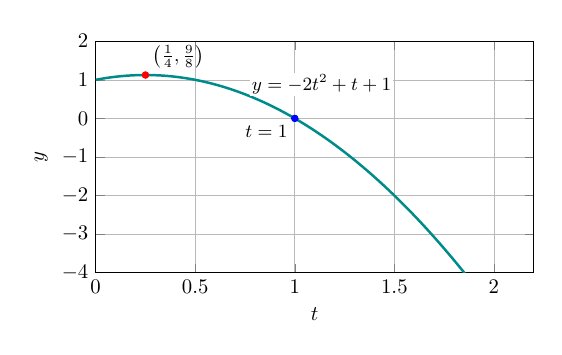
\begin{tikzpicture}[scale=.75]
  \begin{axis}[
    width=9cm,height=5.5cm,
    xmin=0,xmax=2.2,
    ymin=-4,ymax=2,
    domain=0:2.2,
    samples=200,
    xlabel={$t$},ylabel={$y$},
    xtick={0,0.5,1,1.5,2},
    ytick={-4,-3,-2,-1,0,1,2},
    grid=both,
    grid style={line width=.2pt, draw=gray!30},
    major grid style={line width=.3pt,draw=gray!55},
    smooth
  ]
    % 曲线 y=1+t-2t^2
    \addplot[very thick,outermarginfgcolor] {1+x-2*x^2};
    % 标注顶点
    \addplot[mark=*,only marks,mark size=1.6pt,color=red] coordinates {(0.25,1.125)};
    \node[anchor=south west,font=\small] at (axis cs:0.25,1.125) {$\left(\tfrac{1}{4},\tfrac{9}{8}\right)$};
    % 零点 (求解 1+t-2t^2=0 => t=(1\pm\sqrt{1+8})/4=(1\pm3)/4 -> t=1,-1/2)
    \addplot[mark=*,only marks,mark size=1.6pt,color=blue] coordinates {(1,0)};
    \node[anchor=north east,font=\small] at (axis cs:1,0) {$t=1$};
    % 标注函数表达式
    \node[xshift=1cm,anchor=north east,font=\small,fill=white,inner sep=1pt] at (axis cs:1.2,1.2) {$y=-2t^{2}+t+1$};
  \end{axis}
\end{tikzpicture}
\end{center}
\end{exer}%\newpage
\begin{exer}
已知正实数 $a,b$ 满足 $\dfrac{1}{(2a+b)b}+\dfrac{2}{(2b+a)a}=1$,求 $ab$ 的最大值。

\itshape\small
解一:
\begin{flalign*}
&左右同乘以ab得:\dfrac{a}{2a+b}+\dfrac{2b}{2b+a}=ab&\\
&令\begin{cases}
2a+b=m\\
2b+a=n
\end{cases}则:\begin{cases}
a=\dfrac{2m-n}{3}\\
b=\dfrac{2n-m}{3}
\end{cases}\\
&\therefore ab=\dfrac{\dfrac{2m-n}{3}}{m}+\dfrac{2\times\dfrac{2n-m}{3}}{n}=\dfrac{2m-n}{3m}+\dfrac{4n-2m}{3n}=\dfrac{2}{3}+\dfrac{4}{3}-\big(\dfrac{n}{3m}+\dfrac{2m}{3n}\big)\\
&\because \dfrac{n}{3m}+\dfrac{2m}{3n}\ge 2\sqrt{\dfrac{n}{3m}\cdot\dfrac{2m}{3n}}=\dfrac{2\sqrt{2}}{3}\quad(当3n^2=6m^2,即n=\sqrt{2}m,取等)\\
&\therefore ab_{max}=2-\dfrac{2\sqrt{2}}{3}
\end{flalign*}
解二:
\itshape\small\kaishu
\begin{flalign*}
&\therefore ab=\dfrac{1}{2+\dfrac{b}{a}}+\dfrac{2}{2+\dfrac{a}{b}}&\\
&令\dfrac{b}{a}为t(t>0),则原式变为:ab=\dfrac{1}{2+t}+\dfrac{2}{2+\dfrac{1}{t}},显然ab<\dfrac{1}{2}+\dfrac{2}{2}<2\\
&即求\dfrac{1}{2+t}+\dfrac{2}{2+\dfrac{1}{t}}的最大值,为了方便设为K(K=ab,k\in(0,2)),则:\\
&K=\dfrac{1}{2+t}+\dfrac{2}{2+\dfrac{1}{t}}=\dfrac{1}{2+t}+\dfrac{2t}{2t+1}\\
&两边同乘以 (2+t)(2t+1),得\\
& (2+t) (2t+1)=(2t+1)+2t (t+2)\\
&化简,得:(2K-2)t^2+(5K-6)t+2K-1=0\\
&\because 等式成立,方程一定有解\\
&\therefore \Delta=(5K-6)^2-4(2K-2)(2K-1)=9K^2-36K+28\ge 0\\
&\therefore K\ge 2+\dfrac{2\sqrt{2}}{3} 或 K\le 2-\dfrac{2\sqrt{2}}{3}\\
&又\because K\in(0,2)\\
&\therefore K\in(0,2-\dfrac{2\sqrt{2}}{3})\\
&ab的最大值为,2-\dfrac{2\sqrt{2}}{3}
\end{flalign*}
\end{exer}

\begin{exer}[待定系数法]
\\
已知$a,b>0,则\dfrac{ab+b}{a^2+b^2+1}$的最大值?

\itshape\small\noindent
对于$a^2+b^2+c^2$形式,可以利用待定系数法配凑,例如:
\[a^2+b^2+c^2=a^2+\lambda b^2 +(1-\lambda)b^2+c^2\ge2\sqrt{\lambda}ab+2\sqrt{1-\lambda}bc\]
这样就会让a,b,c三者联系起来。把例中的1当作$c^2=1$,则:
\begin{flalign*}
&原式分母\ge 2\sqrt{\lambda}ab+2\sqrt{1-\lambda}b\cdot1&\\
&分子=ab+b,ab项系数为1,b项系数也为1。我们需要对应项成比例:\\
&\dfrac{1}{2\sqrt{\lambda}}=\dfrac{1}{2\sqrt{1-\lambda}}\\
&解得\lambda=\dfrac{1}{2}\\
&\therefore 原式\le\dfrac{ab+b}{\sqrt{2}(ab+b)}=\dfrac{\sqrt{2}}{2}\\
&\therefore 最大值为\dfrac{\sqrt{2}}{2}
\end{flalign*}
\end{exer}

\begin{exer}
已知$a>0,b>0,求\dfrac{ab+b}{a^2+b^2+1}$的最大值。
\end{exer}
利用上例的配凑思想可解。
\begin{exer}
$已知x,y>0,且x+2y+\sqrt{xy}=2,求x+3y的最大值。$
\end{exer}
\kaishu
利用基本不等式可知:$\sqrt{xy}\le\dfrac{x+y}{2}$,原式变为:$2\le x+2y+\dfrac{x+y}{2}$。

此时对比题目要求的结果是x+3y。思考:如何才能让 $x+2y+\dfrac{x+y}{2}$(通过某种变换)$\rightarrow\quad x+3y?$显然$\dfrac{x+y}{2}$中,分子x,y前面有某种系数就可以。

但是的$x+y$是由$\sqrt{xy}$得来的,这是题目给出的条件,我们无法修改,我们应该如何做?

没办法改变条件,但可以对条件进行变形,利用$a\times\dfrac{1}{a}$的特性,把$\sqrt{xy}\rightarrow\sqrt{(a\cdot x) \times\dfrac{y}{a}}$; 由基本不等式得:$\sqrt{(ax) \times\dfrac{y}{a}}\le\dfrac{ax+\dfrac{y}{a}}{2}$

现在的问题就变成如何求出a的值。

原式变形为:$2=x+2y+\sqrt{(ax) \times\dfrac{y}{a}}\le x+2y +\dfrac{ax+\dfrac{y}{a}}{2}=(\dfrac{a}{2}+1)x+(2+\dfrac{1}{2a})y$
对比要求的结果:$x+3y$,$x,y的系数比1:3$

$\therefore \dfrac{\dfrac{a}{2}+1}{2+\dfrac{1}{2a}}=\dfrac{1}{3}\iff 3a^2+2a-1=0$

解得:$a=\begin{cases}
\dfrac{1}{3}\\
-\dfrac{4}{3}
\end{cases}
$

其实这二个解均可使用,但对于基本不等式,如果配的系数为负数,不满足使用条件,麻烦,取$\dfrac{1}{3}$即可。

$\therefore 2= x+2y+\sqrt{(\dfrac{1}{3}x)\times\dfrac{y}{\frac{1}{3}}}=x+2y+\sqrt{\dfrac{x}{3}\times 3y}\le x+2y+\dfrac{\dfrac{x}{3}+3y}{2}=\dfrac{7}{6}x+\dfrac{7y}{2}=\dfrac{7}{6}(x+3y)$

$\therefore x+3y\ge 2\times\dfrac{6}{7}=\dfrac{12}{7}$
%\end{flalign*}

\end{document}
